
%(BEGIN_QUESTION)
% Copyright 2010, Tony R. Kuphaldt, released under the Creative Commons Attribution License (v 1.0)
% This means you may do almost anything with this work of mine, so long as you give me proper credit

An electronic DP transmitter has an input range of 0 to 100 inches water column and an output range of 4 to 20 mA.  When subjected to a series of known pressures (5-point up/down test), it responds as such:

% No blank lines allowed between lines of an \halign structure!
% I use comments (%) instead, so that TeX doesn't choke.

$$\vbox{\offinterlineskip
\halign{\strut
\vrule \quad\hfil # \ \hfil & 
\vrule \quad\hfil # \ \hfil \vrule \cr
\noalign{\hrule}
%
% First row
Applied pressure & Output signal \cr
%
% Another row
(" WC) & (mA) \cr
%
\noalign{\hrule}
%
% Another row
0 & 3.7 \cr
%
\noalign{\hrule}
%
% Another row
25 & 7.9 \cr
%
\noalign{\hrule}
%
% Another row
50 & 12.1 \cr
%
\noalign{\hrule}
%
% Another row
75 & 16.3 \cr
%
\noalign{\hrule}
%
% Another row
100 & 20.5 \cr
%
\noalign{\hrule}
%
% Another row
75 & 16.3 \cr
%
\noalign{\hrule}
%
% Another row
50 & 12.1 \cr
%
\noalign{\hrule}
%
% Another row
25 & 7.9 \cr
%
\noalign{\hrule}
%
% Another row
0 & 3.7 \cr
%
\noalign{\hrule}
} % End of \halign 
}$$ % End of \vbox

Graph this instrument's ideal transfer function on the graph below, along with its {\it actual} transfer function graph based on the measured values recorded above.  Then, determine what kind of calibration error it has ({\it zero shift}, {\it span shift}, {\it linearity}, and/or {\it hysteresis}).

$$\includegraphics[width=15.5cm]{i03730x01.eps}$$


\vfil 

Hint: a computer spreadsheet program might be a useful tool in graphing this instrument's response.  Feel free to attach a printed copy of a spreadsheet graph instead of hand-sketching one on this page.

\underbar{file i03730}
\eject
%(END_QUESTION)





%(BEGIN_ANSWER)

This is a graded question -- no answers or hints given!

%(END_ANSWER)





%(BEGIN_NOTES)

This transmitter definitely has a {\it span} error, and one could say it has a {\it zero} error as well:

$$\includegraphics[width=15.5cm]{i03730x02.eps}$$

If the transmitter only had a zero error, we would see its output be offset from the ideal values by the same amount across its range.  The clue that this error is {\it span} related is how the error keeps progressing by the same amount with every interval along the 0-100\% range.  Note the error figures in this expanded table, particularly how they change by 0.2 mA with every 25\% change in applied pressure:

% No blank lines allowed between lines of an \halign structure!
% I use comments (%) instead, so that TeX doesn't choke.

$$\vbox{\offinterlineskip
\halign{\strut
\vrule \quad\hfil # \ \hfil & 
\vrule \quad\hfil # \ \hfil & 
\vrule \quad\hfil # \ \hfil \vrule \cr
\noalign{\hrule}
%
% First row
Applied pressure & Output signal & Error\cr
%
% Another row
(" WC) & (mA) & (mA) \cr
%
\noalign{\hrule}
%
% Another row
0 & 3.7 & -0.3 \cr
%
\noalign{\hrule}
%
% Another row
25 & 7.9 & -0.1 \cr
%
\noalign{\hrule}
%
% Another row
50 & 12.1 & +0.1 \cr
%
\noalign{\hrule}
%
% Another row
75 & 16.3 & +0.3 \cr
%
\noalign{\hrule}
%
% Another row
100 & 20.5 & +0.5 \cr
%
\noalign{\hrule}
%
% Another row
75 & 16.3 & +0.3 \cr
%
\noalign{\hrule}
%
% Another row
50 & 12.1 & +0.1 \cr
%
\noalign{\hrule}
%
% Another row
25 & 7.9 & -0.1 \cr
%
\noalign{\hrule}
%
% Another row
0 & 3.7 & -0.3 \cr
%
\noalign{\hrule}
} % End of \halign 
}$$ % End of \vbox


%INDEX% Calibration errors, identifying

%(END_NOTES)

